\chapter{GERBIL -- General Entity Annotator Benchmarking Framework}

\graffito{
This chapter introduces GERBIL--a framework for benchmarking semantic annotation systems with the ultimate goal to provide stable, citable URIs for comparable experiments. 
The author of this thesis is the main author of the corresponding publications~\cite{gerbil_demo_2015,GERBIL} and co-author of the demonstration paper~\cite{gerbil_dev_2015} and the technical report~\cite{techreport_gerbil}. 
He co-implemented  and co-evaluated GERBIL together with Michael Röder.
GERBIL won the Best Demo Award 2015 at the Extended Semantic Web Conference.
}
\label{cha:gerbil}

The implementation of the original vision behind the Semantic Web demands the development of approaches and frameworks for the seamless extraction of structured data from text. 
While manifold annotation frameworks have been developed over the last years to address (some of) the sub-tasks related to the extraction of structured data from unstructured data \cite{TagMe2,AIDA,spotlight,milne2008learning,babelfy,piccinno2014tagme,rizzo2014,steinmetz-n-2013-statistical,agdistis_iswc}, the provision of comparable results for these systems remains a tedious problem.
Furthermore, the fair and exhaustive comparison of our own \ac{NED} approach AGDISTIS (Chapter~\ref{cha:agdistis}) to other state-of-the-art approaches illustrated the open \emph{Evaluation Gap} faced by this research field.
The issue of  comparability of results is not to be regarded as being intrinsic to the annotation task. Indeed, it is now well established that scientists spend between 60\% and 80\% of their time preparing data for experiments \cite{GIL2014,jermyn1999preparing,peng2011reproducible}. Data preparation being such a tedious problem in the annotation domain is mostly due to the different formats of the gold standards as well as the different data representations across reference datasets.
%\todo[inline]{AnBo: --change-- different formatting of the textual data in reference datasets --to-- different data representations in reference datasets. Axel:Done}
These restrictions have led to authors evaluating their approaches on datasets (1) that are available to them and (2) for which writing a parser as well as an evaluation setup can be carried out with reasonable effort.
%\todo[inline]{AnBo: easy sounds like an affront, suggestion: is easy --to-- can be implemented within reasonable effort. Axel: Done.} 
In addition, a large number of quality measures have been developed and used actively across the annotation research community to evaluate the same task, leading to the results across publications on the same topics not being easily comparable. For example, while some authors publish macro-F-measures and simply call them F-measures, others publish micro-F-measures for the same purpose, leading to significant discrepancies across the scores. The same holds for the evaluation of how well entities match. Indeed, partial matches and complete matches have been used in previous evaluations of annotation systems \cite{cornolti,FOX}. This heterogeneous landscape of tools, datasets and measures leads to a poor repeatability of experiments, which makes the evaluation of the real performance of novel approaches against the state of the art rather difficult.

Thus, our own and the insights above have led to a movement towards the creation of frameworks to ease the evaluation of solutions that address the same annotation problem~\cite{ERD2014,cornolti}. 
We present GERBIL -- a general entity annotator benchmark --, a community-driven effort to enable the continuous evaluation of annotation approaches. 
GERBIL is an open-source and extensible framework that allows evaluating systems against  \overallGERBILannotators different annotators on \overalldatasets different datasets within 6 different experiment types.\footnote{Numbers are taken from the 2015 publication~\cite{GERBIL}. Current numbers can be found in Section~\ref{sec:currentNumbersForGERBIL}}. 
%At this point in time, GERBIL integrates . Moreover, \overallNrOfMatchingTypes matching types are provided. 
By integrating such a large number of datasets, experiment types and frameworks, GERBIL allows users to evaluate their frameworks against other semantic entity annotation systems (short: entity annotation systems) by using exactly the same setting, leading to fair comparisons based on exactly the same measures. 
While the evaluation core of GERBIL is based on the BAT-framework \cite{cornolti}, our approach goes beyond the state of the art in several respects:
\begin{itemize}
\item GERBIL provides \emph{persistent URLs} for experimental settings. Hence, by using GERBIL for experiments, system developers can ensure that the settings for their experiments (measures, datasets, versions of the reference frameworks, etc.) can be reconstructed in a  unique manner in future works. 
%\item Through experiment URLs, GERBIL also addresses the problem of \emph{archiving} experimental results and allows end users to gather all pieces of information required to choose annotation frameworks for practical applications.
\item GERBIL aims to be a \emph{central repository for annotation results} without being a central point of failure: While we make experiment URLs available, we also provide users directly with their results (via machine-readable data) to ensure that they use them locally without having to rely on GERBIL.
\item The results of GERBIL are published in a \emph{machine-readable format}. In particular, our use of DataID~\cite{dataID} and DataCube~\cite{datacube} to denote frameworks and datasets ensures that results can be easily combined and queried (for example to study the evolution of the performance of frameworks) while the exact configuration of the experiments remains uniquely reconstructable. By these means, we also tackle the problem of \emph{reproducibility}. 
\item Through the provision of results on different datasets of different types and the provision of results on a simple user interface, GERBIL also provides means to quickly gain an overview of the current performance of annotation frameworks, thus providing (1) developers with insights pertaining to the type of data on which their accuracy needs improvement and (2) end users with insights allowing them to choose the right system for the tasks at hand.
\item With GERBIL, we introduce the notion of knowledge base-agnostic benchmarking of entity annotation systems through generalized experiment types. By these means, we allow to benchmark frameworks against a diverse set of reference datasets from any domain grounded in any reference knowledge base. 
\end{itemize}


To ensure that the GERBIL framework is useful to both end users and system developers, its architecture and interface were designed with the following principles in mind:

\begin{itemize}
\item \textbf{Easy integration of annotators}: We provide a wrapping interface that allows annotators to be evaluated via their REST interface. In particular, we integrated \numberOfadditionalAnnotators additional annotators not evaluated against each other in previous works (e.g., \cite{cornolti}).  
\item \textbf{Easy integration of datasets}: We also provide means to gather datasets for evaluation directly from data services such as DataHub.\footnote{\url{http://datahub.io}} In particular, we added \numberOfadditionalDatasets new datasets to GERBIL.
\item \textbf{Easy addition of new measures}: The evaluation measures used by GERBIL are implemented as interfaces. Thus, the framework can be easily extended with novel measures devised by the annotation community.
\item \textbf{Extensibility}: GERBIL is provided as an open-source platform that can be extended by members of the community both to new tasks and different purposes.
\item \textbf{Diagnostics}: The interface of the GERBIL framework was designed to provide developers with means to easily detect aspects in which their tool(s) need(s) to be improved. 
\item \textbf{Portability of results}: We generate human- and machine-readable results to ensure maximum usefulness and portability of the results generated by our framework. 
\end{itemize}


The rest of this chapter presents and evaluates GERBIL. 
%We begin by giving an overview of related work.
First, we present the GERBIL framework.
Especially, we focus in particular on how annotators and datasets can be added to GERBIL and give a short overview of the annotators and frameworks that are currently included in the framework. 
We then present an evaluation of the framework that aims to quantify the effort necessary to include novel annotators and datasets to the framework. 
Finally, we present the current state of GERBIL in Section~\ref{sec:currentNumbersForGERBIL}.
%We conclude with a discussion of the current state of GERBIL and a presentation of future work. 
More information can be found at the project webpage \url{http://gerbil.aksw.org}. % and at the open source code repository page \url{https://github.com/AKSW/gerbil}.
%The online version of GERBIL can be accessed at \url{http://gerbil.aksw.org/gerbil}.


\section{The GERBIL Framework}
\label{sec:architecture}
\begin{figure*}[htb!]
\centering
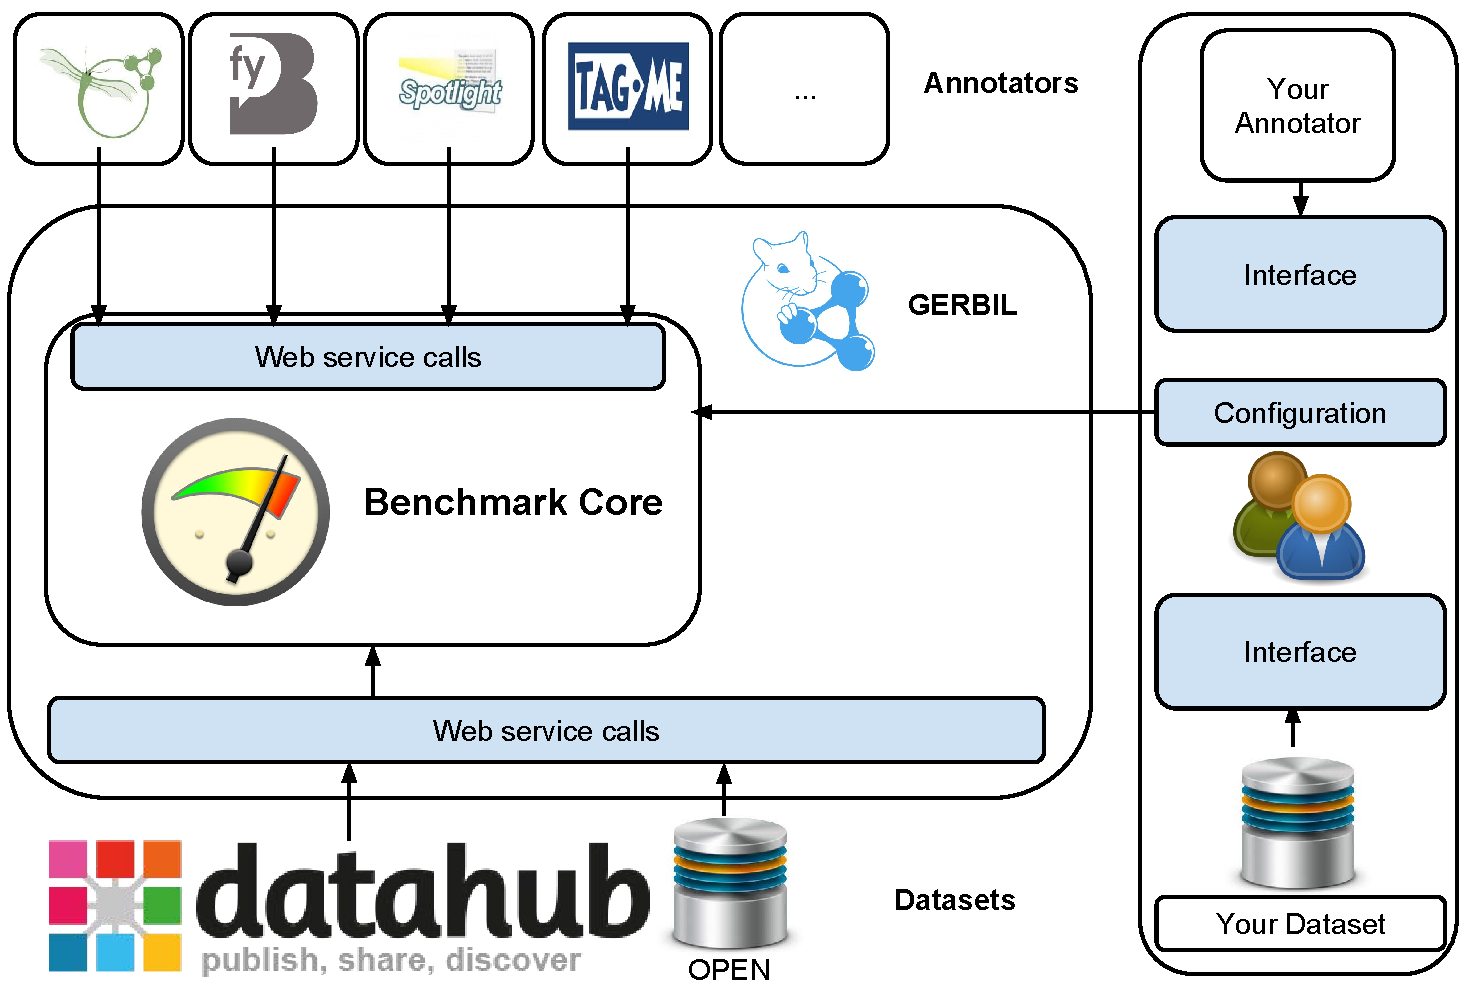
\includegraphics[width=\linewidth]{part_02/benchmarking/WWW_GERBIL/online_annotator_benchmark.pdf}
\caption{Overview of GERBIL's abstract architecture. Interfaces to users and providers of datasets and annotators are marked in blue.
%\todo[inline]{AnBo: Should the arrows/calls triggered from the core \emph{to}\ the datasets?}
}
\label{fig:architecture}
\end{figure*}

%Publishing, reproducing and archiving entity annotation results is a near-impossible endeavour.
%Finding and reusing datasets for comprehensive benchmarks involves often a trem\-endous amount of addition work.

\paragraph{Architecture Overview}
GERBIL abides by the architectural pattern of model-view-controller, see Figure~\ref{fig:architecture}.
Entity annotation systems, datasets and configurations like experiment type, matching or metric are implemented as controller interfaces easily plug-able to the core controller. 
The output of experiments as well as descriptions of the various components are stored in a server-less database for fast deployment. % reachable from each controller. 
Finally, the view component displays configuration options respectively renders experiment results delivered by the central component which is communicating with the interfaces and the database.

%\todo[inline]{AnBo: I have doubts regarding the buzzwords here. 1) A SOA needs a service repository providing callable interfaces to services but do not wrap the service. I am not sure what the actual implementation status is. Maybe we should take over the wording of our SEMANTiCS paper: oriented at the principles of service-oriented architectures. But maybe it is more closely to a plugin-architecture?
%2) Implementing a MVC pattern with distributed services is very complicated. Maybe a MVP pattern is a good description of the actual implementation?}
%\todo[inline]{How does GERBIL work internally? Short description of architecture needed}



% of fine grained measures to be able to cover a wide variety of experiments using diverse NER and \ac{NED} approaches.
%GERBILs core is based on the endeavour of Cornolti et al.'s BAT-Framework~\cite{cornolti} for comparing entity annotation systems. 

%\todo[inline]{(Andrea) We should add a table/image/example to clarify the different setups, even if some of them do not properly belong to the NED/EL/NEL/NER categories such as C2W, Sc2W and Rc2W which do not require the actual mention/entity mapping. Moreover, Sa2W and A2W can be seen as the same task assuming that the score for A2W systems is always equal to 1. (Ricardo): I agree with the last sentence. But that is how it is given in Cornoltis work. Furthermore, I would like to add a table mapping the approaches to categories. What do you think? And maybe add examples to the table below. (Andrea): which kind of categories? I don't think that examples for all the setups are really needed there should be only a single general example to make clear what EL is}
%postponed to M2 paper


\subsection{Experiment Types, Matching, Metrics}
\label{sec:definitions}
%\todo[inline]{@Marco, Paolo/@Ricardo: please proof read this subsection}

%\begin{table*}[th]
\centering
\begin{tabular}{@{}p{3cm}p{2cm}p{3cm}p{7cm}@{}}
\toprule
Problem & Input & Output & Description \\ \midrule


Disambiguate to Wikipedia (D2KB) &
Text, Set of mentions &
Set of relevant annotations &
Assign to each input mention its pertinent entity (possibly null) \\ \midrule

Annotate to Wikipedia (A2KB) &
Text &
Set of relevant annotations &
Identify the relevant mentions in the input text and assign to each of them the pertinent entities \\ \midrule

Scored-annotate to Wikipedia (Sa2KB) &
Text &
Set of relevant and scored annotations &
As A2W, but here each annotation is assigned a score representing the likelihood that the annotation is correct \\ \midrule

Concepts to Wikipedia (C2KB) &
Text &
Set of relevant tags &
Tags are taken as the set of relevant entities that are mentioned in the input text \\ \midrule

Scored concepts to Wikipedia (Sc2KB) &
Text &
Set of relevant and scored tags &
As C2W, but here each tag is assigned a score representing the likelihood that the annotation is correct \\ \midrule

Ranked-concepts to Wikipedia (Rc2KB) &
Text &
Ranked list of relevant tags &
Identify the entities mentioned in a text and rank them in terms of their relevance for the topics dealt with in the
input text\\ \midrule

Classification/Typing to Wikipedia (T2KB) &
 &
 &
\\ \midrule

Entity Salience (ES2KB) &
  &
  &
\\\midrule

Entity Annotation/Detection (A) &
  &
  &
\\
\midrule
Word Sense Disambiguation (WSD) &
  &
  &
\\
\midrule
Relation Extraction (input text, predicate output: triple (BOA?) &
  &
  &\\
\bottomrule
\end{tabular}
\caption{Overview of the different task types.}
\label{tab:tasktypes}
\end{table*}

%\todo[inline]{add a table of mappings from tools to tasks}
%\todo[inline]{@Ricardo,Giuseppe,Micha, Axel: Discuss matchings (esp. TAC-KBP }
%postponed to M2
%\todo[inline]{(Ricardo) we need to discuss how to handle NIL entities while linking step, maybe consider measures from http://jhoff.de/wp-content/papercite-data/pdf/hoffart-2014hp.pdf. \\(Giuseppe) Whenever you refer to NIL then you are touching the TAC KBP EL/EDL effort somehow. There is already a consistent and mature body of work on that. I also encourage you to take a look at http://nlp.cs.rpi.edu/kbp/2014/KBP2014EL\_V1.1.pdf. The metrics proposed in TAC KBP already measure the effect of NIL links.}
%postponed to M2
%Here, we want to point to two import task types, i.e., D2W - disambiguation to Wikipedia which determines for each mention in a given set of mentions its pertinent entity~\cite{Cucerzan07} - and A2W - annotation to Wikipedia  which determines for a given unstructured text a set of relevant entities~\cite{milne2008learning}.
%'These problems can be casted in two main classes: the first consists of three problems which address the identification of (possibly scored) annotations, and thus the identification of mention-entity pairs; the second consists of three further problems that involve finding tags (possibly scored or ranked), thus accounting only for the entities.'
%For a detailed list of problems and their definition please have a look at the article itself~\cite{cornolti}.

Experiments run in our framework can be configured in several manners. In the following, we present some of the most important parameters of experiments available in GERBIL. 

%\paragraph{Experiment types}
An experiment type defines the way used to solve a certain problem when extracting information.
Cornolti et al.'s~\cite{cornolti} BAT-framework offers six different experiment types, namely (scored) annotation (S/A2KB), disambiguation (D2KB) -- also known as \ac{EL} -- and (scored respectively ranked) concept annotation (S/R/C2KB) of texts. 
In~\cite{rizzo2014}, the authors propose two types of experiments, focusing on highlighting the strengths and weaknesses of the analyzed systems.
Thereby, performing \textit{i)} entity recognition, i.e., the detection of the exact match of the pair entity mention and type (e.g., detecting the mention \textit{Barack Obama} and typing it as a \textit{Person}), and \textit{ii)} entity linking, where an exact match of the mention is given and the associated DBpedia URI has to be linked (e.g., locating a resource in DBpedia which describes the mention \textit{Barack Obama}).
This work differs from the previous one for experimenting in entity recognition, and on annotating entities to a \ac{RDF} \ac{KB}.

GERBIL reuses the six experiments provided by the BAT-framework and extends them by the idea to not only link to Wikipedia but to any knowledge base $K$.
%Thereby, we extend the idea of the before mentioned frameworks by introducing the concept of knowledge base-agnostic benchmarks.
%\todo[inline]{The following sentence does not make sense to me}
%That is, datasets and annotators are aware of their underlying knowledge bases, e.g., Wikipedia, DBpedia, Babelnet etc..
One major formal update of the measures in GERBIL is that in addition to implementing experiment types from previous frameworks, it also measures the influence of NIL annotations, i.e., the linking of entities that are recognized as such but cannot be linked to any resource from the reference knowledge base $K$. For example, the string \texttt{Barack Obama} can be recognized as a person name by several frameworks but cannot be linked to Wikipedia/DBpedia, as Ricardo does not have a URI in these reference datasets. 
Our framework extends the experiments types of~\cite{cornolti} as follows: Let $m=(s,l,d,c) \in M$ denote an entity mention in document $d \in D$ with start position $s$, length $l$ and confidence score $c \in [0,1]$.
%that links to either a resource from the resource knowledge base $K$ or a global NIL entity if the entity mentioned is not in $K$. 
Note that some frameworks might not return (1) a position $s$ or a length $l$ for a mention, in which case we set $s=0$ and $l=0$; (2) a score $c$, in which case we set $c=1$.


We implement six types of experiments:
\begin{enumerate}
\item \textbf{D2KB}: The goal of this experiment type is to map a set of \emph{given} entity mentions (i.e., a subset $\mu \subseteq M$) to entities from a given \ac{KB} or to NIL. Formally, this is equivalent to finding a mapping $a: \mu \rightarrow K \cup \{NIL\}$. In the classical setting for this task, the start position, the length and the score of the mentions $m_i$ are not taken into consideration. 
%The document for each entity is given explicitly. That's part of the formalization
%\todo[inline]{Micha: I don't understand the second sentence. Why is everything set to 0?. Axel: Fixed}
\item \textbf{A2KB}: This task is the classical \ac{NER}/\ac{NED} task, thus an extension of the D2KB task. Here two functions are to be found. First, the entity mentions need to be extracted from a document set $D$. To this end, an extraction function $ex: D \rightarrow 2^M$ must be computed. The aim of the second step is then to match the results of $ex$ to entities from $K \cup \{NIL\}$\footnote{For $NIL$ entities, annotators and gold standards should generate URIs to cope with entities which are not in a KB. Based on this assumption, GERBIL will be able to support in-document respectively cross-document co-referencing experiments in the future.} by devising a function $a$ as in the D2KB task.
%\todo[inline]{AnBo: I suggest a formal definition: $akin: m \rightarrow e$, where $e \in K \cup \{NIL\}$.Axel: akin is not a function}
%i.e.,  mapping a document $d$ to a set of entities $e_i \in K$ belonging to certain mentions $m_i(s_i,l_i)$ of this document. Formally, this is a mapping $a: d \rightarrow K \cup \{NIL\}$. The scores for those entities are ignored and thus $c_i=0$.
\item \textbf{Sa2KB}:
Sa2KB is an extension of A2KB where the scores $c_i \in [0,1]$ of the mentions detected by the approach are taken into consideration. These scores are then used during the evaluation to find an optimal threshold maximizing the target measures~\cite{cornolti}.
\item \textbf{C2KB}: The concept tagging task C2KB aims to detect entities when given a document. Formally, the tagging function $tag$ simply returns a subset of $K$ for each input document $d$.
\item \textbf{Sc2KB}: This task is an extension of C2KB where the tagging function returns a set $K^* = |{(k,s)|k\in K, s \in[0,1]|}$ for each input document $d$.
\item \textbf{Rc2KB}: In this particular extension of C2KB, the tagging function returns a sorted list of resources from $K$. %, i.e., an element of $K^*$, where $K^* = \bigcup\limits_{i=0}^\infty K^i$. 
\end{enumerate}

\begin{comment}
\begin{align}
\begin{split}
D2KB:&(d,K,\{m_1,\ldots,m_n\}) \rightarrow \{a_1,\ldots,a_n|\\
&a_i=(m_i,e_i), e_i\in K\cup\emptyset\}
\end{split}\\
\begin{split}
A2KB:&(d,K) \rightarrow \{a_1,\ldots,a_n|\\
&a_i=(s_i,l_i,e_i), e_i\in K\cup\emptyset, 0 < s_i \le |d|,\\
&0 < l_i, (s_i + l_i) \le |d|\}
\end{split}\\
\begin{split}
Sa2KB:&(d,K) \rightarrow \{a_1,\ldots,a_n|\\
&a_i=(s_i,l_i,e_i,c_i), e_i\in K\cup\emptyset, 0 < s_i \le |d|,\\
&0 < l_i, (s_i + l_i) \le |d|, 0 \le c_i \leq 1\}
\end{split}\\
\begin{split}
C2KB:&(d,K) \rightarrow \{e_1,\ldots,e_n|\\
&e_i\in K\cup\emptyset\}
\end{split}\\
\begin{split}
Rc2KB:&(d,K) \rightarrow \{a_1,\ldots,a_n|\\
&a_i=(e_i,r_i),e_i\in K\cup\emptyset,r \in [0,1]\}
\end{split}\\
\begin{split}
Sc2KB:&(d,K) \rightarrow \{a_1,\ldots,a_n|\\
&a_i=(e_i,c_i), e_i\in K\cup\emptyset, 0 \le c_i \leq 1\}
\end{split}
\end{align}
\end{comment}

With this extension, our framework can now deal with gold standard datasets and annotators that link to any \ac{KB}, e.g., DBpedia, BabelNet~\cite{babelnet} etc., as long as the necessary identifiers are URIs.
We were thus able to implement \numberOfadditionalDatasets new gold standard datasets usable for each experiment type, cf. Section~\ref{sec:datasets}, and \numberOfadditionalAnnotators new annotators linking entities to any \ac{KB} instead of solely Wikipedia like in previous works, cf. Section~\ref{sec:annotators}.
With this extensible interface, GERBIL can be extended to deal with supplementary experiment types, e.g., entity salience~\cite{cornolti}, entity detection~\cite{FOX}, typing~\cite{rizzo2014}, word sense disambiguation (WSD)~\cite{babelfy}, co-reference resolution~\cite{CETUS_2015} and relation extraction~\cite{FOX}.
These categories of experiment types will be added to GERBIL in further versions, see Section~\ref{sec:currentNumbersForGERBIL}.

%GERBIL leverages Linked Data usages for Benchmarks.

\paragraph{Matching}

A matching defines which conditions the result of an annotator has to fulfill to be a correct result.
In case of existing redirections, we assume an implicit matching function to account for the many-to-one relation~\cite{cornolti}.
The first matching type $M$ used for the C2KB, Rc2KB and Sc2KB experiments is the \textit{strong entity matching}.
Here, each mention is mapped to an entity of the knowledge base $K$ via a matching function $f$ with $f(m) \in K \cup \{NIL\}$.
Following this matching, a single entity mention $m = (s, l, d, c)$ returned by the annotator is correct iff it matches exactly with one of the entity mentions $m' = (s', l', d, c')$ in the gold standard $G(d)$ of d~\cite{cornolti}. Formally,
\begin{align}
M(m,G)=
\begin{cases}
1 &  \text{iff }\exists m' \in G, f(m) = f(m'), \\
0 & \text{else.}
\end{cases}
\end{align}

For the D2KB experiments, the matching is expanded to the \textit{strong annotation matching} and includes the correct position of the entity mention inside the document.
\begin{align}
M_e(m,G) =
\begin{cases}
1 &  \text{iff }\exists m' \in G: f(m) = f(m') \wedge s = s' \wedge \\
  &l = l', \\
%&\quad s_g = s_a, l_g = l_a\\
0 & \text{else.}
\end{cases}
\end{align}

The strong annotation matching can be used for A2KB and Sa2KB experiments, too.
However, in practice this exact matching can be misleading.
A document can contain a gold standard named entity like "President Barack Obama" while the result of an annotator only marks "Barack Obama" as named entity.
Using an exact matching leads to weighting this result as wrong while a human might rate it as correct.
Therefore, the \textit{weak annotation matching} relaxes the conditions of the strong annotation matching.
Thus, a correct annotation has to be linked to the same entity and must overlap the annotation of the gold standard.

\begin{align}
M_w (m,G)=
\begin{cases}
1 &  \text{iff }\exists m' \in G, f(m) = f(m')  \land (\\
 &\ \ \ \,\, ( s \leq s' \land (s+l) \leq (s'+l') )\\ % left overlap
 &\ \ \lor ( s \geq s' \land (s+l) \geq (s'+l') )\\ % right overlap
 &\ \ \lor ( s \leq s' \land (s+l) \geq (s'+l') )\\ % outer overlap
 &\ \ \lor ( s \geq s' \land (s+l) \leq (s'+l') ))\\ % inner overlap
0 & \text{else.}
\end{cases}
\end{align}

%\todo[inline]{(RU) TAC-KBP?}
%postponed to M2

\paragraph{Metrics}
GERBIL offers six measures subdivided into two groups and derived from the BAT-framework, namely the micro- and the macro-group of precision, recall and F-measure.
%That is, macro measures are defined as average overall documents of the corresponding group measures while micro measures are calculated document-wise and averaged thereafter~\cite{cornolti}.
Those measures ignored NIL annotations, i.e., if a gold standard dataset contains entities that are not contained in the target knowledge base $K$ and an annotator detects the entity and links it to any URI, emerging novel URI or NIL, this will always result in a false-positive evaluation. 
This behavior changed since version 1.2.0 when GERBIL's new own and independent evaluation core was published, see \url{https://github.com/AKSW/gerbil/wiki/URI-matching}.
To alleviate this problem, GERBIL allows adding additional measures to evaluate the results of annotators regarding the heterogeneous landscape of gold standard datasets, see Section~\ref{sec:currentNumbersForGERBIL}.

\subsection{Annotators}
\label{sec:annotators}

GERBIL aims to reduce the amount of work required to compare existing as well as novel annotators in a comprehensive and reproducible way. To this end, we provide two main approaches to evaluating entity annotation systems with GERBIL.
\begin{enumerate}
\item \textbf{BAT-framework Adapter}
Within BAT, annotators can be implemented by using a Java-based wrapper interface.
Since GERBIL is based on the BAT-framework, annotators of this framework can be added to GERBIL easily.
Due to the community effort behind GERBIL, we could raise the number of published annotators from 5 to \overallGERBILannotators.
We investigated the effort to implement a BAT-framework adapter in contrast to evaluation efforts done without a structured evaluation framework in Section~\ref{cha332:sec:eval}.

\item \textbf{NIF-based Services}:
GERBIL provides implementation means to understand NIF-based~\cite{NIF} communication over Web service in two ways.
First, if the server-side implementation of annotators understands NIF-documents as input and output format, GERBIL and the framework can simply exchange NIF-documents.\footnote{We describe the exact requirements to the structure of the NIF document on our project webpage's wiki as NIF offers several ways to build a NIF-based document or corpus.}
%we can use a more simple and unified approach to bind new annotators into GERBIL.
Thus, novel NIF-based annotators can be deployed efficiently into GERBIL and use a more robust communication format compared to the amount of work necessary for deploying and writing a BAT-framework adapter.
%\todo[inline]{Here, I would argue that the implementation of a single NIF-Web service is faster than deploying the BAT-framework and implementing a BAT-framework adapter.}
Second, if developers do not want to publish their APIs or write source code, GERBIL offers the possibility for NIF-based Web services to be tested online by providing their URI and name only\footnote{\url{http://gerbil.aksw.org/gerbil/config}}. 
GERBIL does not store these connections in terms of API keys or URLs but still offers the opportunity of persistent experiment results.
%This web-based interface leverages the implementation of future annotators by offering a royalty-free annotation standard\footnote{\url{http://persistence.uni-leipzig.org/nlp2\ac{RDF}/}}.
\end{enumerate}

GERBIL offers \overallGERBILannotators entity annotation systems with a variety of features, capabilities and experiments.
In the following, we present current state-of-the-art approaches both available or unavailable in GERBIL.
%For a list of available Web services, see Table~\ref{tab:annotator}.

%sorted by year
\begin{enumerate}
\item \textbf{Cucerzan}: As early as in 2007, Cucerzan presented a \ac{NED} approach based on Wikipedia~\cite{Cucerzan07}. The approach tries to maximize the agreement between contextual information of input text and a Wikipedia page as well as category tags on the Wikipedia pages.
The test data is still available\footnote{\url{http://research.microsoft.com/en-us/um/people/silviu/WebAssistant/TestData/}} but since we can safely assume that the Wikipedia page content changed a lot since 2006, we do not use it in our framework, nor we are aware of any publication reusing this data.
Furthermore, we were not able to find a running Web service or source code for this approach.

\item \textbf{Wikipedia Miner}: This approach was introduced in~\cite{milne2008learning} in 2008 and is based on different facts like prior probabilities, context relatedness and quality, which are then combined and tuned using a classifier.
The authors evaluated their approach based on a subset of the AQUAINT dataset\footnote{\url{http://www.nist.gov/tac/data/data_desc.html\#AQUAINT}}.
They provide the source code for their approach as well as a Web service\footnote{\url{http://wikipedia-miner.cms.waikato.ac.nz/} is out-of-service since 15th February 2016.} which is available in GERBIL.

\item \textbf{Illinois Wikifier}: In 2011, ~\cite{rat:rot} presented an \ac{NED} approach for entities from Wikipedia. 
In this article, the authors compare local approaches, e.g., using string similarity, with global approaches, which use context information and lead finally to better results.
The authors provide their datasets\footnote{\url{http://cogcomp.cs.illinois.edu/page/resource_view/4}} as well as their software\footnote{\url{http://cogcomp.cs.illinois.edu/page/software_view/33}} online.
Since the Illinois Wikifier is currently only available as local binary and GERBIL is solely based on Web services, we excluded it from GERBIL for the sake of comparability and server load.

\item \textbf{DBpedia Spotlight}: One of the first semantic approaches~\cite{spotlight}\ was published in 2011, this framework combines \ac{NER} and \ac{NED} approach based upon DBpedia\footnote{\url{https://github.com/dbpedia-spotlight/dbpedia-spotlight/wiki/Known-uses}}. 
%and acting as a central point for the Semantic Web community
Based on a vector-space representation of entities and using the cosine similarity, this approach has a public (NIF-based) Web service\footnote{\url{https://github.com/dbpedia-spotlight/dbpedia-spotlight/wiki/Web-service}} as well as its online available evaluation dataset\footnote{\url{http://wiki.dbpedia.org/spotlight/isemantics2011/evaluation}}.

\item \textbf{TagMe 2}: TagMe 2~\cite{TagMe2} was publised in 2012 and is based on a directory of links, pages and an inlink graph from Wikipedia.
The approach recognizes named entities by matching terms with Wikipedia link texts and disambiguates the match using the in-link graph and the page dataset.
Afterwards, TagMe 2 prunes identified named entities which are considered as non-coherent to the rest of the named entities in the input text.  
The authors publish a key-protected Web service\footnote{\url{http://tagme.di.unipi.it/}} as well as their datasets\footnote{\url{http://acube.di.unipi.it/tagme-dataset/}} online.
The source code, licensed under Apache 2 licence can be obtained directly from the authors.
%Unfortunately, their approach has two drawbacks: 
%(1) Texts with more than 3000 characters are a problem for the Web service. 
%Thus we slice longer texts near 3000 although there is the danger of cutting a named entity.
The datasets comprise only fragments of 30 words or less of full documents. 
Thus, we decided that these datasets will not be part of GERBIL. 
%\todo[inline]{drawback (1) is obselete as soon as we change to POST (2) is not a drawback directly.}

\item \textbf{AIDA}: The AIDA approach~\cite{AIDA} relies on coherence graph building and dense subgraph algorithms and is based on the YAGO2\footnote{\url{http://www.mpi-inf.mpg.de/yago-naga/yago/}} \ac{KB}.
%Specifically, this approach uses dense sub-graphs to identify coherent mentions using a greedy algorithm enabling Web scalability. 
Although the authors provide their source code, a Web service and their dataset which is a manually annotated subset of the 2003 CoNLL shared task~\cite{conll2003}, GERBIL does not use the Web service since it is not stable enough for regular replication purposes.\footnote{\url{https://www.mpi-inf.mpg.de/departments/databases-and-information-systems/research/yago-naga/aida/}}

\item \textbf{NERD-ML}: In 2013,~\cite{vanErp2013} proposed an approach for entity recognition tailored for extracting entities from tweets. The approach relies on a machine learning classification of the entity type given a rich feature vector composed of a set of linguistic features, the output of a properly trained Conditional Random Fields classifier~\cite{Lafferty:2001:CRF:645530.655813} and the output of a set of off-the-shelf \ac{NER} extractors supported by the NERD Framework. The follow-up, NERD-ML~\cite{rizzo2014}, improved the classification task by re-designing the selection of the features, and they proposed experiments on both microposts and newswire domains.
NERD-ML has a public Web service which is part of GERBIL\footnote{\url{http://nerd.eurecom.fr/}}.


%too long in comparision
\item \textbf{KEA NER/NED}: This approach is the successor of the approach introduced in~\cite{steinmetz-n-2013-statistical} which is based on a fine-granular context model taking into account heterogeneous text sources %, as e.g. user tags, natural language texts, 
as well as text created by automated multimedia analysis. %, as e.g. automated speech recognition, optical character recognition, or visual concept detection. 
The source texts can have different levels of accuracy, completeness, granularity and reliability which influence the determination of the current context. 
Ambiguity is solved by selecting entity candidates with the highest level of probability according to the predetermined context. 
The new implementation begins with the detection of groups of consecutive words (n-gram analysis) and a lookup of all potential DBpedia candidate entities for each n-gram. 
The disambiguation of candidate entities is based on a scoring cascade. % including the analysis of connected components in the entity candidates' spanning sub-graphs in DBpedia, co-occurrence analysis with Wikipedia article texts, graph popularity measures (in-degree, pagerank)~\cite{dbpedia-graphmeasures}, as well as statistical and string distance metrics. 
%The final decision on the most likely entity candidate is determined with the help of machine learning classifiers, which is subject of current research. 
KEA is available as NIF-based Web service\footnote{\url{http://s16a.org/kea}}.


\item \textbf{WAT}: WAT is the successor of TagME~\cite{TagMe2}.\footnote{\url{http://github.com/nopper/wat}}
%, developed by Piccinno et al.~\cite{piccinno2014tagme} and was presented during the ERD Challenge~\cite{carmel2014erd}. 
%The project is released as an open source library\footnote{\url{http://github.com/nopper/wat}}. % and it is written in Scala. 
The new annotator includes a re-design of all TagME components, namely, the spotter, the disambiguator, and the pruner. 
Two disambiguation families were newly introduced: graph-based algorithms for collective entity linking based % (i.e., exploiting well-known graph algorithms such as PageRank, HITS and SALSA) 
and vote-based algorithms for local entity disambiguation (based on the work of Ferragina et al.~\cite{TagMe2}). 
The spotter and the pruner can be tuned using SVM linear models. 
Additionally, the library can be used as a D2KB-only system by feeding appropriate mention spans to the system. 
%commented because cornolti said it is not true. The system inherits some of the limitation of the legacy TagME~\cite{TagMe2}, i.e., being optimized for short texts. % (i.e. the spotter and the pruner modules are responsible for introducing many of the false positives).

\item \textbf{AGDISTIS}: This approach~\cite{agdistis_iswc} is a pure entity disambiguation approach (D2KB) based on string similarity measures, an expansion heuristic for labels to cope with co-referencing and the graph-based HITS algorithm.
The authors published datasets\footnote{\url{https://github.com/AKSW/n3-collection}} along with their source code and an API\footnote{\url{https://github.com/AKSW/AGDISTIS}}.
AGDISTIS can only be used for the D2KB task.

\item \textbf{Babelfy}: The core of this approach lies in the use of random walks and a densest subgraph algorithm to tackle the word sense disambiguation and entity linking tasks in a multilingual setting~\cite{babelfy} thanks to the BabelNet semantic network~\cite{babelnet}.
Babelfy has been evaluated using six datasets: three from earlier SemEval tasks \cite{pradhan2007semeval,NavigliLH:2007,Naviglietal:13}, one from a Senseval task \cite{snyder2004english} and two already used for evaluating AIDA \cite{AIDA,HoffartSNTW:2012}.
All of them are available online but distributed throughout the Web. 
Additionally, the authors offer a Web service limited to 100 requests per day which are extensible for research purposes\footnote{\url{http://babelfy.org}} \cite{BabelfyAPI}.

%\todo[inline]{@diego(?): describe DEXTER here, and update all tables}

\item \textbf{Dexter}: This approach \cite{ceccarelli2013dexter} is an open-source implementation of an entity disambiguation framework.
The system was implemented in order to simplify the implementation of an entity linking approach and allows to replace single parts of the process.
%It runs on commodity hardware and requires only 3 gigabytes of memory.
The authors implemented several state-of-the-art disambiguation methods.
Results in this paper are obtained using an implementation of the original TagMe disambiguation function.
Moreover, Ceccarelli et al. provide % the source code\footnote{\url{http://dexter.isti.cnr.it}} as well as 
a Web service.
\end{enumerate}



Table~\ref{tab:annotator} compares the implemented annotation systems of GERBIL and the BAT-Framework.
While AGDISTIS has been in the source code of the BAT-Framework provided by a third-party after publication of Cornolti et al.'s initial work~\cite{cornolti} in 2014, GERBIL's community effort led to the implementation of overall \numberOfadditionalAnnotators new annotators as well as the before mentioned generic NIF-based annotator.
The AIDA annotator as well as the Illinois Wikifier are not available in GERBIL\footnote{\url{GERBIL version 1.0.0}} since we restrict ourselves to Web services.
However, these algorithms as well as upcoming annotation systems can be integrated at any time as soon as their Web services are available, see Section~\ref{sec:currentNumbersForGERBIL}.


\begin{table}[htb!]
\centering
\begin{tabular}{llccc}
\toprule
                                        && \textbf{BAT-Framework}           & \textbf{GERBIL}                    & \textbf{Experiment Type}\\
\midrule
\cite{milne2008learning}		&Wikipedia Miner	& \haken 					& \haken	&	SA2KB\\
\cite{rat:rot}							&Illionois Wikifier	& \haken 					& (\haken) 	& 	SA2KB\\
\cite{spotlight}						&Spotlight           	& \haken                 & \haken  & SA2KB\\
\cite{TagMe2}						&TagMe 2           	& \haken                 & \haken	& SA2KB\\
\cite{AIDA}							&AIDA                	& \haken                 & (\haken)	& SA2KB\\
%&van Erp?                                &                         & ?                         &\\
\cite{steinmetz-n-2013-statistical}			&KEA                	&                         		& \haken	& SA2KB\\
\cite{piccinno2014tagme}	&WAT            		&                         		& \haken 	& SA2KB\\
\cite{agdistis_iswc}				&AGDISTIS           & (\haken)               & \haken	& D2KB\\
\cite{babelfy}						&Babelfy              &                         		& \haken	& SA2KB\\
\cite{rizzo2014}					&NERD-ML          	&                         		& \haken 	& SA2KB\\
\cite{ceccarelli2013dexter}	&Dexter 				&          					& \haken 	& SA2KB\\
											&NIF-based Annotator       &             	& \haken  & any\\
\bottomrule
\end{tabular}
\caption{Overview of implemented annotator systems. Brackets indicate the existence of the implementation of the adapter but also the inability to use it in the live system.}
\label{tab:annotator}
\end{table}

\subsection{Datasets}
\label{sec:datasets}

Table~\ref{tab:corpus_stats} shows the diversity of datasets used for prior evaluations while Table~\ref{tab:datasets} presents an overview of the datasets that were used to evaluate some well-known entity annotators in previous works.
These tables make clear that the numbers and types of used datasets vary a lot, thus preventing a fast comparison of annotation systems.

%GERBIL's main goal is the improvement of the reproducibility of entity annotation experiments. 
%Thus, our approach offers the opportunity to easily compare a wealth of entity annotations systems and various datasets with diverse experiment and matching types as well as metrics, cf. .
%\begin{table}[htb]
\centering
\begin{tabulary}{\columnwidth}{LCC}
\toprule
Dataset                 & Format    & Experiment\\
\toprule
ACE2004                 & MSNBC     & Sa2KB\\
Wiki                    & $\star$   & Sa2W \\
Aquaint                 & $\star$   & Sa2KB\\
MSNBC                   & MSNBC     & Sa2KB\\
IITB                    & XML       & Sa2KB\\
Meij                    & TREC      & Rc2W \\
AIDA/CoNLL              & CoNLL     & Sa2KB \\
N$^3$ collection        & NIF/RDF   & Sa2KB \\
KORE 50                 & NIF/RDF   & Sa2KB \\
Wiki-Disamb30           & tab-separated & Sa2KB \\
Wiki-Annot30            & tab-separated & Sa2KB \\
Spotlight Corpus        & NIF/RDF   & Sa2KB \\
SemEval-2013 task 12    & XML/$\star$&WSD/Sa2KB\\
SemEval-2007 task 7     & XML/$\star$&WSD\\
SemEval-2007 task 17    & XML/$\star$&WSD\\
Senseval-3              & XML/$\star$&WSD\\
Microposts2014          & Microposts2014 & Sa2KB\\
\bottomrule
\end{tabulary}
\caption{Datasets and their formats. A $\star$ indicates various inline or keyfile annotation formats. The experiments follow their definition in Section~\ref{sec:definitions}}
\label{tab:datasetformats}
\end{table}

\begin{table}[tb!]
     \resizebox{\textwidth}{!}{ 
    \begin{tabular}{lp{0.25cm}rp{0.25cm}rp{0.25cm}rp{0.25cm}rp{0.25cm}r}
     \toprule
     \textbf{Corpus} && \textbf{Topic} &&\textbf{Format} && \multicolumn{1}{c}{\textbf{Size}} && \multicolumn{1}{c}{\textbf{Avg. Entity/Doc.}} \\
    \midrule
ACE2004          && news        && MSNBC        &&   57 &&   4.44\\
AIDA/CoNLL       && news        && CoNLL     && 1393 &&  19.97\\
Aquaint          && news        &&  -        &&   50 &&  14.54\\
IITB             && mixed       && XML       &&  103 && 109.22\\
KORE 50          && mixed       && NIF/RDF   &&   50 &&   2.86\\
Meij             && tweets      && TREC          &&  502 &&   1.62\\
Microposts2014   && tweets      &&  -        && 3505 &&   0.65\\
MSNBC            && news        && MSNBC     &&   20 &&  32.50\\
N$^3$ Reuters-128&& news        && NIF/RDF   &&  128 &&   4.85\\
N$^3$ RSS-500    && RSS-feeds   && NIF/RDF   &&  500 &&   0.99\\
Spotlight Corpus && news        && NIF/RDF   &&   58 &&   5.69\\
%Wiki             && encyclopedic    &&   ? &&   ?\\
	\bottomrule
	\end{tabular}}
	\centering
    \caption{Features of the data sets and their documents. Every dataset can be used for the Sa2KB experiment except Meij which is only suitable for the Rc2KB experiment family.}
	\label{tab:corpus_stats}
\end{table}

\begin{table}[tb!]
\centering
 \resizebox{\textwidth}{!}{ 
\begin{tabular}{lccccccccccccccccccc|cc}
\toprule
                   & \rot{Year} & \rot{ACE} & \rot{Wiki} & \rot{Aquaint} & \rot{MSNBC} & \rot{IITB} & \rot{Meij} & \rot{AIDA/CoNLL} & \rot{N$^3$ collection} & \rot{KORE 50} & \rot{Wiki-Disamb30} & \rot{Wiki-Annot30} & \rot{Spotlight Corpus} & \rot{SemEval-2013 task 12} & \rot{SemEval-2007 task 7} & \rot{SemEval-2007 task 17} & \rot{Senseval-3} & \rot{NIF-based corpus} & \rot{Microposts2014} & \rot{Software available?} & \rot{Web service available?} \\ \midrule
Cucerzan & 2007 & & & & \haken & & & & & & & & & & & & & & & \\
%Wikipedia Miner gets a new line --> we put it in two lines to center the cells vertically
Wikipedia & \multirow{2}{*}{2008} & & & \multirow{2}{*}{\haken*} & & & & & & & & & & & & & & & & & \multirow{2}{*}{\haken} \\
Miner &&&&&&&&&&&&&&&&&&&&&\\
\mbox{Illionois Wikifier} & 2011 & \haken & \haken & \haken* & \haken & & & & & & & & & & & & & & & \haken & \\
Spotlight & 2011 & & & & & & & & & & & & \haken & & & & & & & \haken & \haken \\
AIDA & 2011 & & & & & & & \haken & & & & & & & & & & & & \haken & \haken** \\
TagMe 2  & 2012 & & & & & & & & & & \haken & \haken & & & & & & & & \haken & \haken \\
Dexter & 2013 & & & & & & & & & & & & & & & & & & & \haken & \haken \\
KEA & 2013 & & & & & & & & & & & & & & & & & & &  & \haken \\
WAT & 2013 & & & & & & & & & & & & & & & & & & &  \haken & \haken \\

AGDISTIS & 2014 & & & \haken & \haken & \haken & \haken & \haken & \haken & \haken & & & \haken & & & & & & & \haken & \haken \\
Babelfy & 2014 & & & & & & & \haken & & \haken & & & & \haken & \haken & \haken & \haken & & & & \haken \\
\mbox{NERD-ML} & 2014 & & & & & & & \haken & & & & & & & & & & & \haken & \haken & \haken \\
\midrule
BAT- & \multirow{2}{*}{2013} & \multirow{2}{*}{\haken} & \multirow{2}{*}{\haken} & \multirow{2}{*}{\haken} & \multirow{2}{*}{\haken} & \multirow{2}{*}{\haken} & \multirow{2}{*}{\haken} & \multirow{2}{*}{\haken*} & & & & & & & & & & & & \multirow{2}{*}{\haken} & \\
\mbox{Framework} &&&&&&&&&&&&&&&&&&&&&\\
NERD & \multirow{2}{*}{2014} & & & & & & \multirow{2}{*}{\haken} & \multirow{2}{*}{\haken} & & & & & & & & & & & \multirow{2}{*}{\haken} & \multirow{2}{*}{\haken} & \multirow{2}{*}{\haken} \\
\mbox{Framework} &&&&&&&&&&&&&&&&&&&&&\\
GERBIL & 2014 & \haken & \haken & \haken & \haken & \haken & \haken & \haken* & \haken & \haken &  & & \haken &  & & & & \haken & \haken  & \haken & \haken \\ 
\bottomrule
\end{tabular}
}
\caption{Comparison of annotators and datasets with indication whether software or datasets respectively Web services are available for reproduction. $*$ indicates that only a subset has been used to evaluate this annotator.
$**$ indicate that the Web service is not meant to be used within scientific evaluations due to unstable backends.}
\label{tab:datasets}
\end{table}

BAT allows the evaluation of the performance of different a\-ppro\-aches using five datasets, namely AQUAINT, MSNBC, IITB, Meij and AIDA/CoNLL.
With GERBIL, we activate one more dataset already implemented by the authors, namely ACE2004 from Ratinov et al.~\cite{rat:rot}.
Furthermore, we implemented a dataset wrapper for the Microposts2014 corpus which has been used to evaluate NERD-ML~\cite{rizzo2014}. 
The dataset itself was introduced in 2014~\cite{Cano2014} and consists of 3500 tweets especially related to event data.
Moreover, we capitalize upon the uptake of publicly available, NIF based corpora over the last years~\cite{steinmetz-n-2013-statistical,n3}\footnote{\url{http://datahub.io/dataset?license_id=cc-by&q=NIF}}.
To this end, GERBIL implements a Java-based NIF~\cite{NIF} reader and writer module which enables loading arbitrary NIF document collections, as well as the communication to NIF-based Web services.
Additionally, we integrated four English NIF corpora, i.e., the RSS-500 and reuters-128 dataset~\cite{n3}, as well as the Spotlight Corpus and the KORE 50 dataset\footnote{\url{http://www.yovisto.com/labs/ner-benchmarks/}}. 

The extensibility of the datasets in GERBIL is furthermore ensured by allowing users to upload or use already available NIF datasets from DataHub. 
GERBIL will regularly check whether new corpora are available and publish them for benchmarking after a manual quality assurance cycle which ensures their usability for the implemented configuration options.
Additionally, users can upload their NIF-corpora directly to GERBIL avoiding their publication in publicly available sources.
This option allows for rapid testing of entity annotation systems with closed source or licenced datasets.

Some of the datasets shown in Table~\ref{tab:datasets} are either not yet implemented due to size and server load limitations, i.e., Wiki-Disamb30 and Wiki-Annot30, or due their original experiment type.
In particular, the Senseval-3 as well as the different SemEval datasets demand as experiment type word sense disambiguation and thereby linking to BabelNet or Wordnet~\cite{wordnet}, which is not yet covered in GERBIL.
Still, GERBIL offers currently \overalldatasets state-of-the-art datasets reaching from newswire and twitter to encyclopedic corpora of various amounts of texts and entities.
Due to license issues we are only able to provide downloads for 9 of them directly but we provide instructions to obtain the others on our project wiki.

Table~\ref{tab:corpus_stats} depicts the features of the current datasets available in GERBIL, see Section~\ref{sec:currentNumbersForGERBIL} for an overview of the current state of GERBIL datasets.
These provide a broad evaluation ground leveraging the possibility for sophisticated system diagnostics.

%\todo[inline]{@AKSW:  output statistics for all available corpora, i.e., nr of docs, nr of entities, length of documents, domain as table thx.}

%\begin{table}[tb!]
%    \begin{tabular}{lp{0.25cm}rp{0.25cm}rp{0.25cm}r}
%     \toprule
%     \textbf{Corpus} && \textbf{Topic} && \multicolumn{1}{c}{$\left|\text{Documents}\right|$} && \multicolumn{1}{c}{\textbf{Avg. Entity/Doc.}} \\
%    \midrule
%ACE2004          && news            &&   57 &&   4.44\\
%AIDA/CoNLL       && news            && 1393 &&  19.97\\
%Aquaint          && news            &&   50 &&  14.54\\
%IITB             && mixed           &&  103 && 109.22\\
%KORE 50          && mixed           &&   50 &&   2.86\\
%Meij             && tweets          &&  502 &&   1.62\\
%Microposts2014   && tweets          && 3505 &&   0.65\\
%MSNBC            && news            &&   20 &&  32.50\\
%N$^3$ Reuters-128&& news            &&  128 &&   4.85\\
%N$^3$ RSS-500    && RSS-feeds       &&  500 &&   0.99\\
%Spotlight Corpus && news            &&   58 &&   5.69\\
%%Wiki             && encyclopedic    &&   ? &&   ?\\
%	\bottomrule
%	\end{tabular}
%	\centering
%    \caption{Features of the datasets and their documents.}
%	\label{tab:corpus_stats}
%\end{table}




\subsection{Datastructures for Datasets}
\label{cha334:sec:datastructures}

GERBIL unifies the different formats used by existing datasets and annotators.
To this end, GERBIL's interfaces are mainly based on the \emph{NLP Interchange Format} (NIF)~\cite{ISWC2013NIF}.
This is a \ac{RDF}-based Linked Data serialization which provides several advantages such as interoperability by standardization or query-ability.
The \emph{NIF-standard} assigns each document an URI as starting point and generates another Linked Data resource per semantic entity.
Each document is a resource of type \texttt{nif:Context} and its content is the literal of its \texttt{nif:isString} predicate. 
Every entity is an own resource with a newly generated URI pointing to the original document via the \texttt{nif:referenceContext} predicate.
Additionally the begin (\texttt{nif:beginIndex}) and end position (\texttt{nif:endIndex}) as well as the disambiguated URI (\texttt{itsrdf:taIdentRef}) and the respective \ac{KB} (\texttt{itsrdf:taSource}) are stored.
The paramount position of NIF amongst corpora serialisation formats is evident by the growing number of available datasets~\cite{GERBIL}.

%\subsection{Experiment configuration}
%
%%\begin{wrapfigure}{l}{6cm}
%\begin{figure}
%\centering
%\includegraphics[width=0.95\linewidth]{part_02/benchmarking/ESWC_GERBIL_demo/screenshot}
%\caption{Experiment configuration screen.}
%\label{cha333:fig:screenshot}
%\end{figure}
%GERBIL allows for a detailed configuration of an experiment. 
%First, an experiment type defines the way used to solve a certain problem when extracting information.
%Second, GERBIL offers diffrent types of matching, see above.
%(3) \emph{Weak annotation matching $M_w$} has been introduced to relax certain cases. For example,  a gold standard contains a named entity "President Barack Obama" while the result of an annotator only marks "Barack Obama" as named entity. Using an exact matching leads to weighting this result as wrong while a human might rate it as correct. Thus, a correct annotation has to be linked to the same entity and must overlap the annotation of the gold standard.
%(3) \emph{Weak annotation matching $M_w$} relaxes the condition of $M_a$ regarding the position of the entity to allow overlap with the annotation of the gold standard.
%The selection and an explanation of the types of matching for given experiments will be part of the demo (see Figure~\ref{cha333:fig:screenshot}). %\todo[inline]{AN: Add ref to figure as requested above.}

\subsection{Workflow}
%\begin{figure}
%\centering
%\includegraphics[width=0.7\linewidth]{part_02/benchmarking/WWW_GERBIL/screenshot}
%\caption{Experiment configuration screen.}
%\label{cha333:fig:screenshot}
%\end{figure}
%Figure \ref{cha334:fig:architecture} shows the architecture of GERBIL with the data sets at the bottom, the annotators in the top and the user interface as well as user defined annotator and data set at the right.
%A GERBIL session starts at the configuration screen, see Figure~\ref{cha333:fig:screenshot}, with which a user defines the experiment he is interested in.
Each experiment is divided into tasks.
A task comprises the evaluation of a single annotator using a single data set, is encapsulated into a fault-tolerant class and runs inside an own thread.
Our fault-tolerance classes at two types of errors: (1) an annotator may return error codes for single documents, e.g., because of the missing ability to handle special characters.
While other evaluation frameworks tend to cancel the experiments after an exception thrown by the annotator, GERBIL counts these smaller errors and reports them as part of the evaluation result.
The second type of fault tolerance aims at (2) larger errors, e.g., the data set couldn't be loaded or the annotator is unreachable via its Web service.
These run-time errors are handled by storing one of the predefined error codes inside the experiment database.
Therewith, we ensure that the user gets instant feedback if some parts of the experiment couldn't be performed as expected.

During a task, the single documents of a data set are sent to the annotator.
After finishing the last document, the responses are evaluated.
Currently, the evaluation is focused on the quality, i.e., precision, recall, F1-score and error counts, but can be extended.
Moreover, a runtime is also available~\cite{GERBIL}.
For some experiment types, e.g., the entity-linking tasks, the evaluation needs additional information.
GERBIL is able to search for \texttt{owl:sameAs} links to close the gap between data sets and annotators that are based on different knowledge bases.
Currently, this search is mainly based on the information inside the data set and retrieval of the entity mentioned by the annotator.
The search could be extended by using local search indexes that contain mappings between well-known knowledge bases, e.g., DBpedia and Freebase.
%The results are currently written to an HSQL database\footnote{\url{http://hsqldb.org/}}.


\subsection{Experiment Output}
\label{sec:output}

\begin{table}[tb!]
    \begin{tabular}{lcr}
    \toprule
    Annotator & Dataset & F1-micro \\
    \midrule
    DBpedia Spotlight & IITB & 0.444 \\
    Babelfy & IITB & 0.377 \\
    NERD-ML & IITB & 0.488 \\
    WAT & IITB & 0.202 \\
    DBpedia Spotlight & KORE50 & 0.265 \\
    Babelfy & KORE50 & 0.476 \\
    NERD-ML & KORE50 & 0.238 \\
    WAT & KORE50 & 0.523 \\
	\bottomrule
	\end{tabular}
	\centering
    \caption{Results of an example experiment from the 10th November 2014 (\url{http://gerbil.aksw.org/gerbil/experiment?id=201411100001})}
	\label{tab:persistentURL}
\end{table}

GERBIL's main aim is to provide comprehensive, reproducible and publishable experiment results.
Hence, GERBIL's experimental output is represented as a table containing the results, as well as embedded JSON-LD\footnote{\url{http://www.w3.org/TR/json-ld/}} \ac{RDF} data using the RDF DataCube vocabulary~\cite{datacube}.
We ensure a detailed description of each component of an experiment as well as machine-readable, interlinkable results following the 5-star Linked Data principles.
Moreover, we provide a persistent and time-stamped URL for each experiment, see Table~\ref{tab:persistentURL}.


\emph{RDF DataCube} is a vocabulary standard and can be used to represent fine-grained multidimensional, statistical data which is compatible with the  Linked SDMX~\cite{LinkedSDMX} standard. 
Every GERBIL experiment is modelled as \texttt{qb:Dataset} containing the individual runs of the annotators on specific corpora as \texttt{qb:Observations}. 
Each observation features the \texttt{qb:Dimensions} experiment type, matching type, annotator, corpus and time. 
The six evaluation measures offered by GERBIL as well as the error count are expressed as \texttt{qb:Measures}. 
To include further metadata, annotator and corpus dimension properties link \emph{DataID}~\cite{dataID} descriptions of the individual components. 

GERBIL uses DataID~\cite{dataID} ontology that combines VoID~\cite{void} and DCAT~\cite{dcat} metadata with Prov-O~\cite{prov-o} provenance information and ODRL~\cite{odrl} licenses to describe datasets.
Besides metadata properties like titles, descriptions and authors, the source files of the open datasets themselves are linked as \texttt{dcat:Distributions}, allowing direct access to the evaluation corpora. 
Furthermore, ODRL license specifications in \ac{RDF} are linked via \texttt{dc:license}, potentially facilitating automatically adjusted processing of licensed data by \ac{NLP} frameworks. 
Licenses are further specified via \texttt{dc:rights}, including citations of the relevant publications. 

To describe annotators in a similar fashion, we extended DataID for services. 
The class \texttt{Service}, to be described with the same basic properties as dataset, was introduced. 
To link an instance of a \texttt{Service} to its distribution the \texttt{datid:distribution} property was introduced as super property of \texttt{dcat:distribution}, i.e., the specific URL the service can be queried at.
Furthermore, Services can have a number of \texttt{datid:Parameters} and \texttt{datid:Configurations}.
Datasets can be linked via \texttt{datid:input} or \texttt{datid:output}. 
An example JSON-LD is depicted in Listing~\ref{lst:jsonld}.


\begin{figure}[ht!]
\begin{lstlisting}[label=lst:jsonld, caption=Example JSON-LD for an GERBIL experiment.]
{
  "@graph" : [ {
    "@id" : "http://gerbil.aksw.org/gerbil/experiment?id=...\#experiment_...",
    "@type" : [ "gerbil:Experiment", "qb:Dataset" ],
    "experimentType" : "gerbil:A2KB",
    "matching" : "gerbil:WeakAnnoMatch",
    "structure" : "gerbil:dsd",
    "label" : "Experiment 201503160001"
  }, {
    "@id" : "http://gerbil.aksw.org/gerbil/experiment?id=...\#experiment_..._task_0",
    "@type" : "qb:Observation",
    "annotator" : "http://gerbil.aksw.org/gerbil/dataId/corpora/Babelfy",
    "dataset" : "http://gerbil.aksw.org/gerbil/dataId/annotators/ACE2004",
    "statusCode" : "-1",
    "timestamp" : "2015-03-16T12:31:52.469Z"
  } ],
  "@context" : {
    ...
  }
}
\end{lstlisting}
\end{figure}


\subsection{Diagnostics}
\begin{figure}[htb!]
\centering
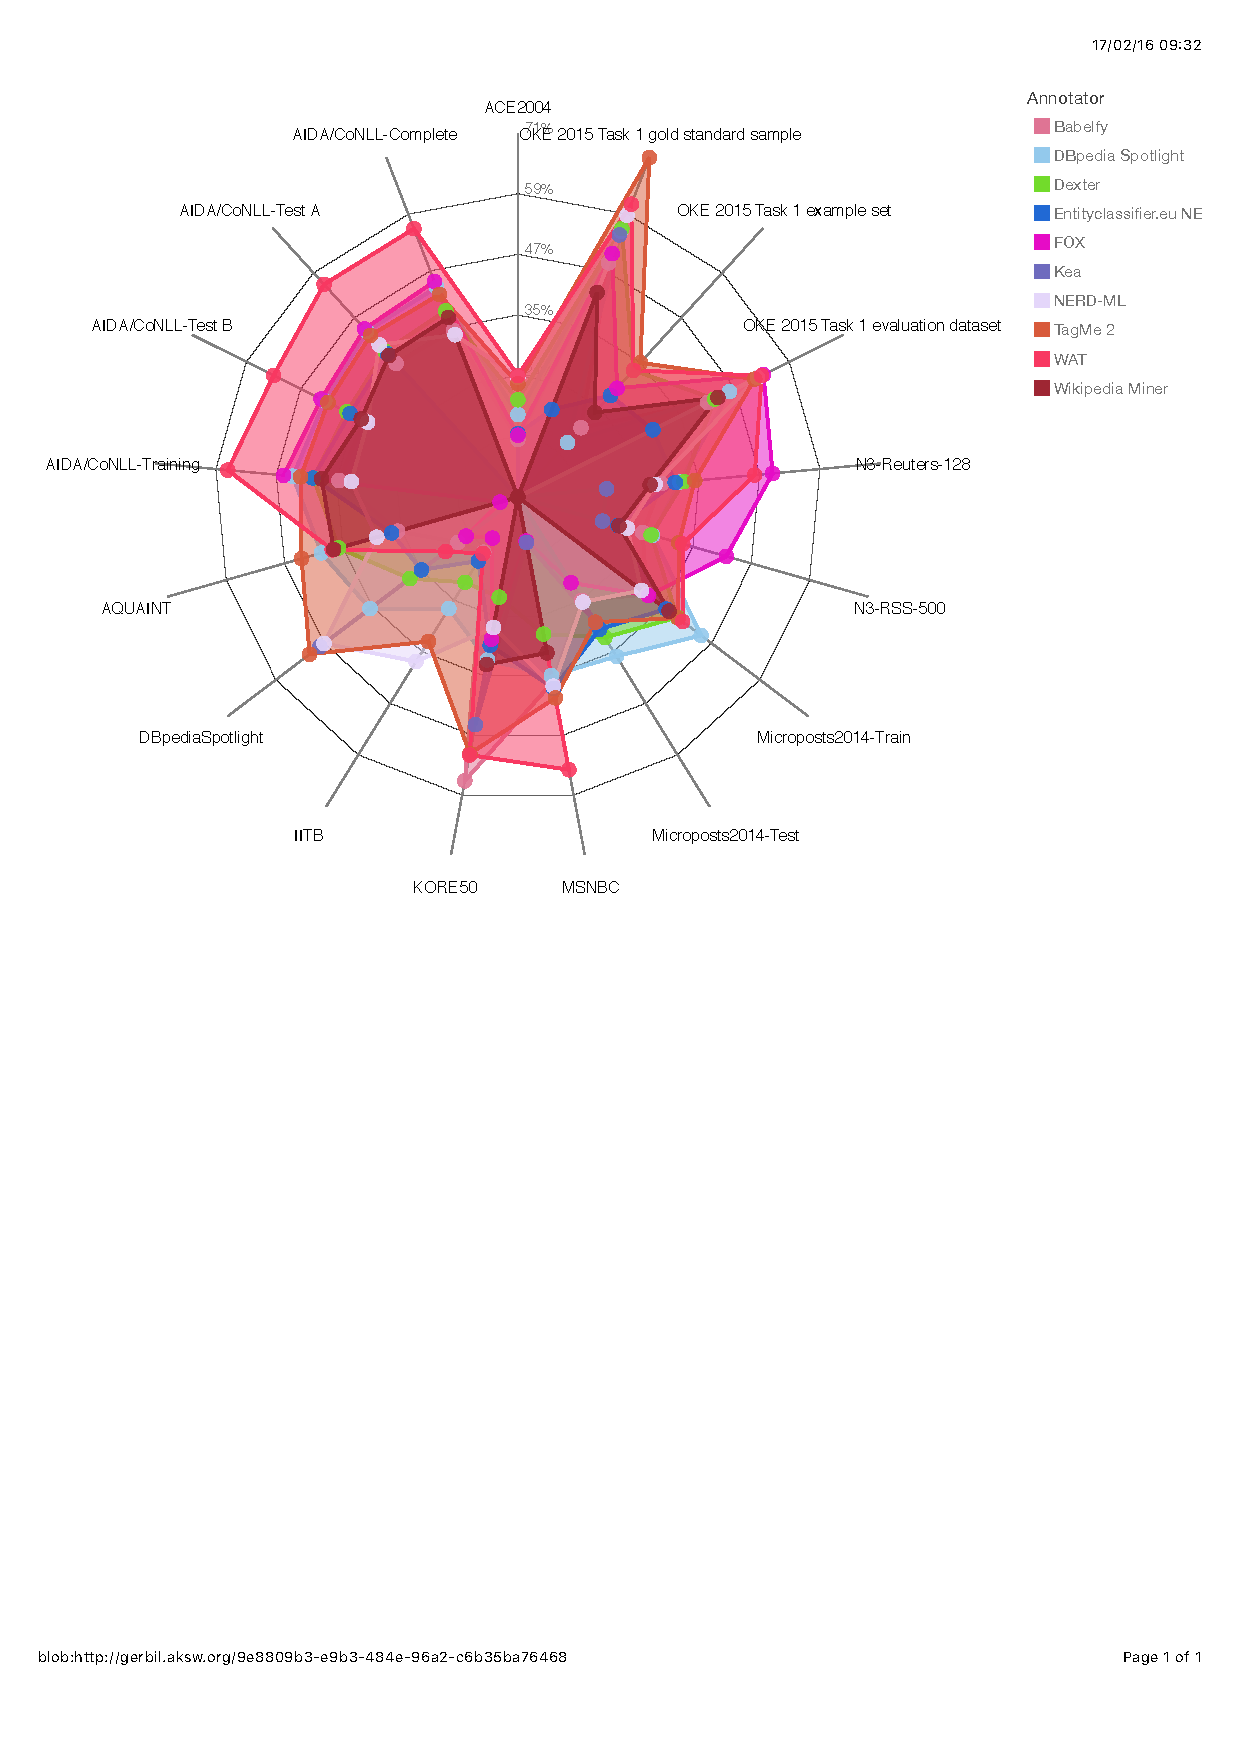
\includegraphics[trim=10 400 10 40,clip,scale=0.7]{part_02/benchmarking/WWW_GERBIL/new_spider_annotators.pdf}
\caption{Example spider diagram of recent A2KB experiments with weak annotation matching.}
\label{cha333:fig:spiderfmeasure}
\end{figure}

\begin{figure}[htb!]
\centering
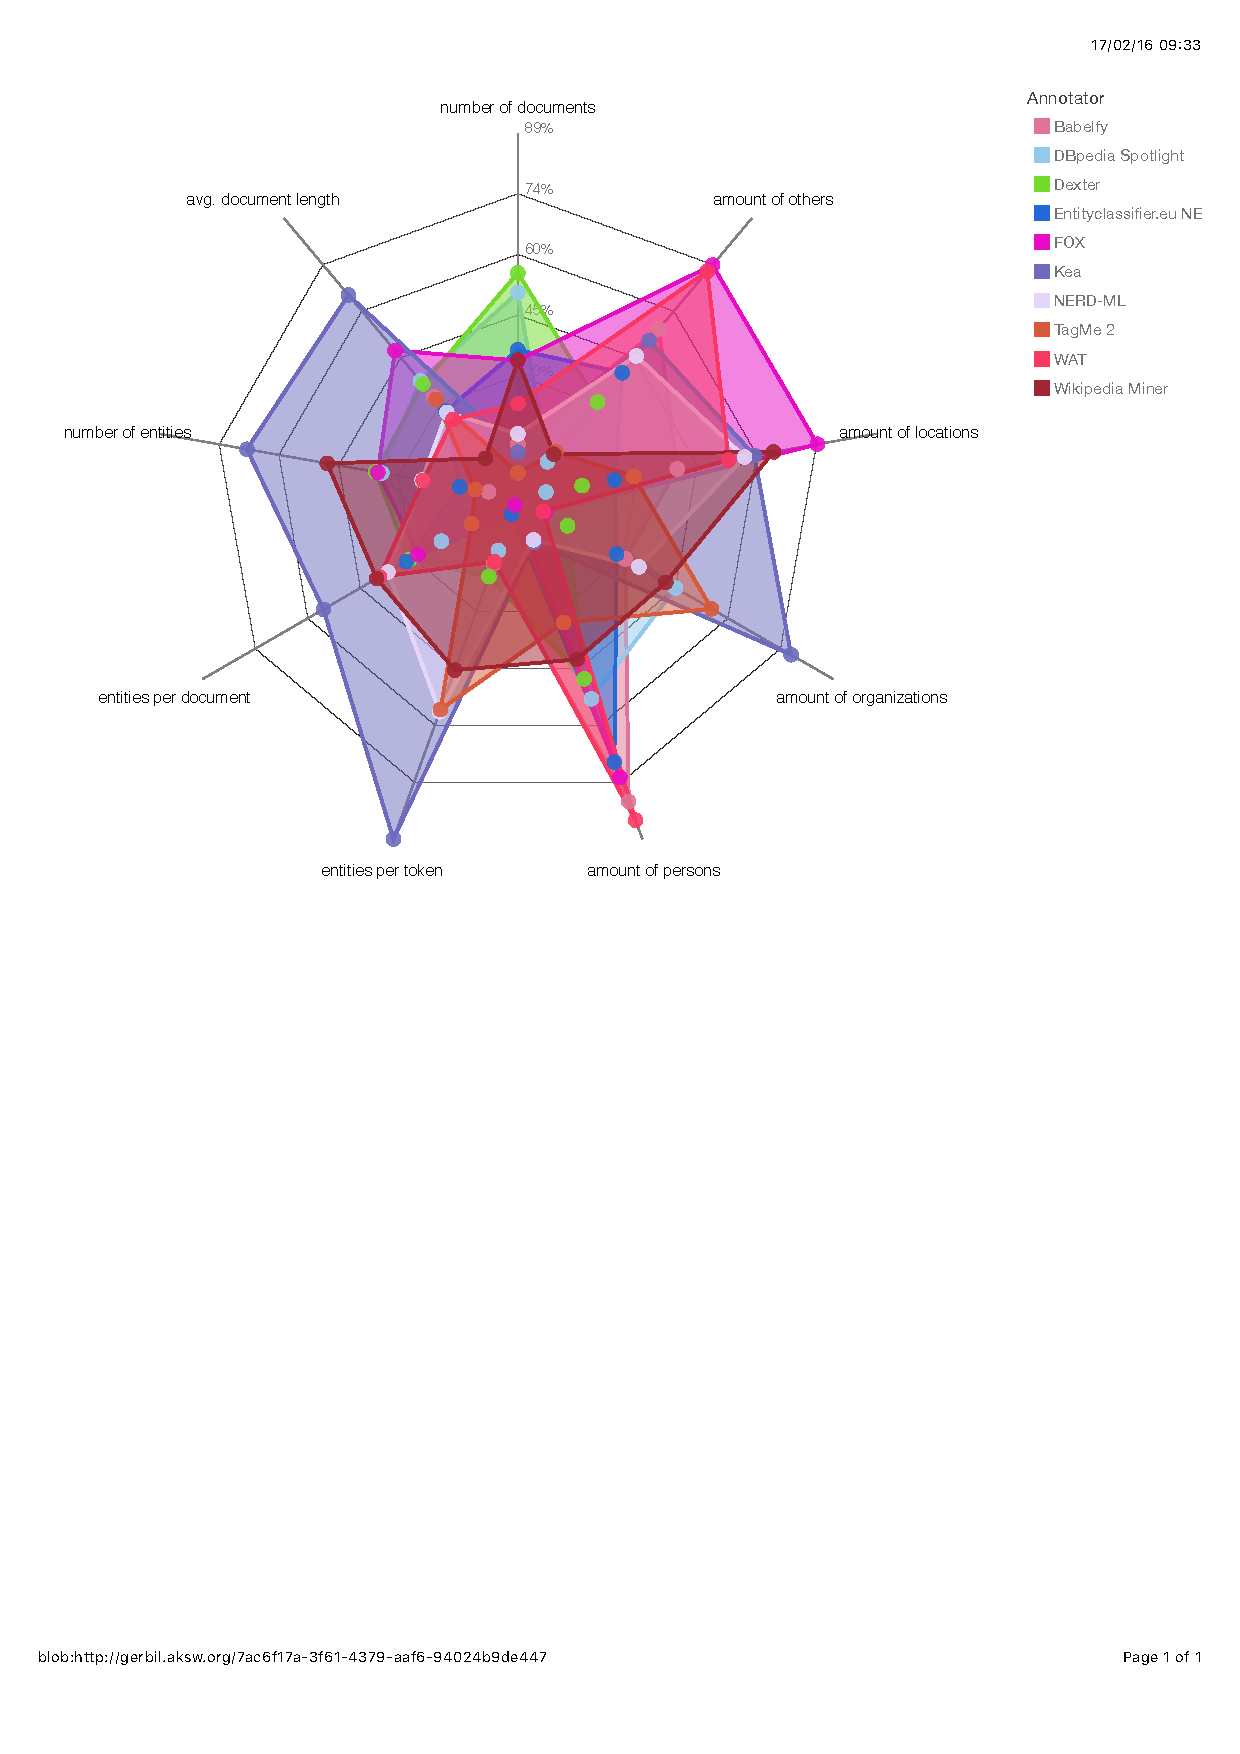
\includegraphics[trim=10 400 10 40,clip,scale=0.7]{part_02/benchmarking/WWW_GERBIL/new_spider_features.pdf}
\caption{Example spider diagram of correlations between annotation results and data set features.}
\label{cha333:fig:spidercorrelations}
\end{figure}

Offering such detailed and structured experimental results opens new research avenues in terms of systems and dataset diagnostics to increase decision makers' ability to choose the right settings for the right use case.
Next to individual configurable experiments, GERBIL offers an overview of recent experiment results belonging to the same experiment and matching type in the form of a table as well as sophisticated visualizations\footnote{\url{http://gerbil.aksw.org/gerbil/overview}}, for instance see Figure~\ref{cha333:fig:spiderfmeasure}. 
This allows for a quick comparison of frameworks and datasets on recently run experiments without additional computational effort.

 As shown in Figure~\ref{cha333:fig:spiderfmeasure}, these results are displayed using interactive spider diagrams that allow the user to easily (1) get an overview of the performance of single tools, (2) compare tools with each other and (3) gather information on the performance on tools on particular data sets.
Furthermore, end users can make use of these results to select the right system for their current requirements. Currently, we display correlations with the following data set features: (1) number of documents and (2) number of entities in the data set, (3) entities per document, (4) entities per token, (5) average length of a document as well as (6) the number  of entities of the different types (persons, locations, organizations, etc.). The interface provides these scores by using spider diagrams akin to those used to display the evaluation metrics, see Figure~\ref{cha333:fig:spidercorrelations}.



%\begin{figure}[htb]
%\centering
%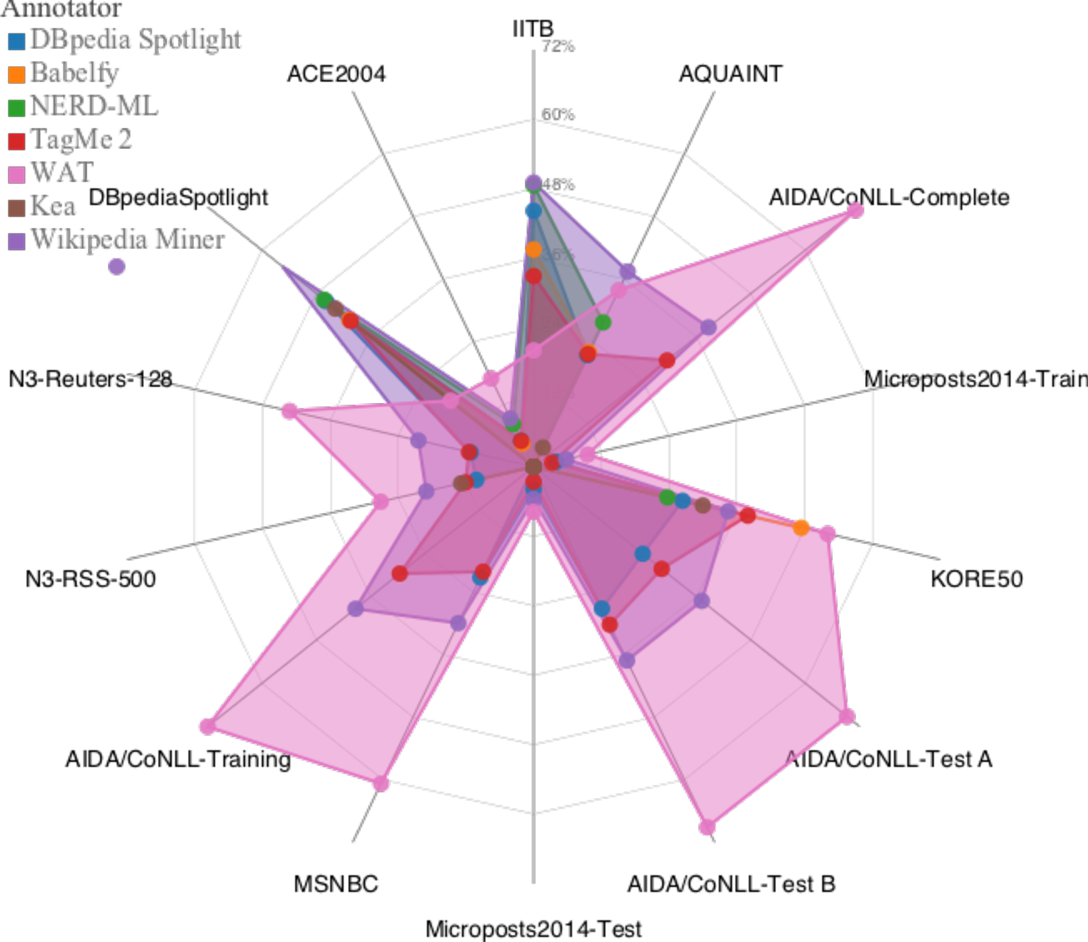
\includegraphics[width=0.5\textwidth]{part_02/benchmarking/WWW_GERBIL/spider}
%\caption{Example spider diagram of recent A2KB experiments with strong annotation matching derived from our online interface}
%\label{fig:spider}
%\end{figure}
%\todo[inline]{For each spider, say when it was pulled}


\section{Evaluation}
\label{cha332:sec:eval}
%GERBIL allows publishing, citing, reproducing and analysing entity annotation experiment data.

To ensure the practicability and convenience of the GERBIL framework, we investigated the effort needed to use GERBIL for the evaluation of novel annotators.
To achieve this goal, we surveyed the workload necessary to implement a novel annotator into GERBIL compared to the implementation into previous diverse frameworks.

Our survey comprised five developers with expert-level programming skills in Java. Each developer was asked to evaluate how much time he/she needed to write the code necessary to evaluate his/her framework on a new dataset.

%\todo[inline]{Add diagram showing time for own data/time on GERBIL}
\begin{figure}[htb!]
\centering
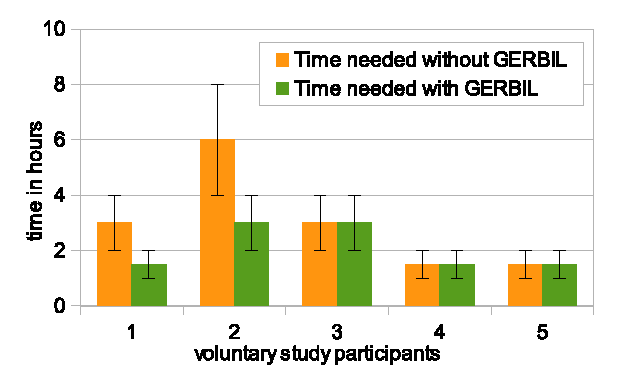
\includegraphics[scale=1]{part_02/benchmarking/WWW_GERBIL/user_study.eps}
\caption{Comparison of effort needed to implement an adapter for an annotation system with and without GERBIL.}
\label{ref:comparedTime}
\end{figure}
%%\todo[inline]{Add diagram showing time for own data/time on GERBIL}
\begin{figure}
\centering
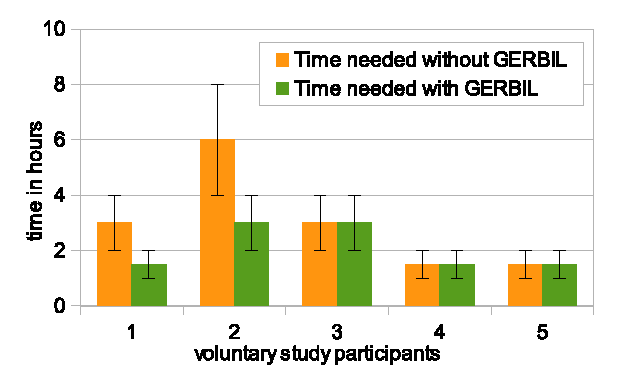
\includegraphics[width=\columnwidth]{part_02/benchmarking/WWW_GERBIL/user_study.eps}
\caption{Comparison of effort needed to implement an adapter for an annotation system with and without GERBIL.}
\label{ref:comparedTime}
\end{figure}


Overall, the developers reported that they needed between 1 and 4 hours to achieve this goal (4x 1-2h, 1x 3-4h), see Figure~\ref{ref:comparedTime}.
Importantly, all developers reported that they needed either the same or even less time to integrate their annotator into GERBIL.
This result in itself is of high practical significance as it means that by using GERBIL, developers can evaluate on (currently) \overalldatasets datasets using the same effort they needed for 1, which is a gain of more than 1100\%.
Moreover, all developers reported they felt comfortable---4 points on average on a 5-point Likert scale between very uncomfortable (1) and very comfortable (5)---implementing the annotator in GERBIL.
Further developers were invited to complete the survey, which is available at our project website.
%\url{ https://docs.google.com/spreadsheets/d/1v3EyAnHxA3zgfoL4CcqEM4_EbvpKiCWeg6qc3FOKf2o/edit#gid=414618098}
Even though small, this evaluation suggests that implementing against GERBIL does not lead to any overhead. On the contrary, GERBIL significantly improves the time-to-evaluation by offering means to benchmark and compare against other annotators respectively datasets within the same effort frame previously required to evaluate on a single dataset.

An interesting side-effect of having all these frameworks and datasets in a central framework is that we can now benchmark the different frameworks with respect to their runtimes within exactly the same experimental settings. These results are of practical concern for end users of annotation frameworks as they are most commonly interested in both the runtime and the quality of solutions. For example, we evaluated the runtimes of the different approaches in GERBIL for the A2KB experiment type on the MSNBC dataset. The results of this experiment are shown in Figure~\ref{fig:runtime}.


\begin{figure}[htb!]
\centering
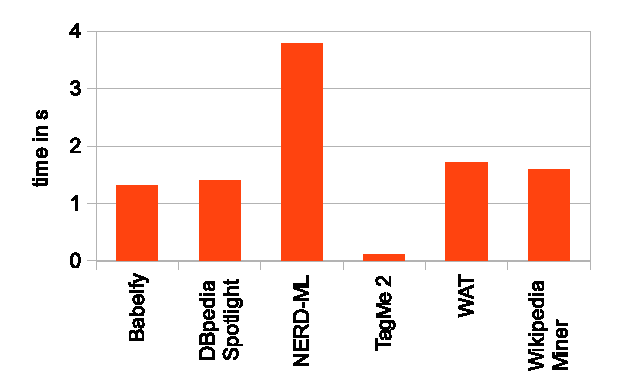
\includegraphics[scale=1]{part_02/benchmarking/WWW_GERBIL/needed_times.eps}
\caption{Runtime per document of different approaches in GERBIL for the A2KB experiment type on the MSNBC dataset.}
\label{fig:runtime}
\end{figure}
%\todo[inline]{@Micha runtime in s/document?}

%\subsection{Reproducibility of experiments}
%\label{sec:repro}
%\todo[inline]{ADD A2W, D2W benchmark tables here with URIs to proof GERBIL %works.}
%The main goal of GERBIL is to provide comprehensible experiments in the field of NER and NED.
%Especially, we are interested in reproducing the results of AGDISTIS~\cite{agdistis_iswc}, TagMe 2~\cite{TagMe2,Cornolti} and Babelfy~\cite{babelfy}.
\section{Current development of GERBIL}
\label{sec:currentNumbersForGERBIL}


Recently, we released the latest version 1.2.2 of GERBIL~\cite{techreport_gerbil}\footnote{\url{https://github.com/AKSW/gerbil/releases/tag/v1.2.2}}.
Here, we present the novel additions to GERBIL and explain which impact our framework had to the community.

\paragraph{Types and Improved Diagnostics}
Since the initial release of GERBIL, we added four tasks to the list of available experiment types. 
First, we supported the OKE Challenge 2015~\cite{okechallenge} by adding the first and second task, i.e, named entity recognition, typing and linking as well as entity type annotation (cf. CETUS~\cite{CETUS_2015}), to GERBIL's experiments types.
Here, we also integrated a hierarchical f-measure for the evaluation of the new typing task. 
The challenge requirements led to the introduction of the new concept of sub-tasks.
Thus, users are now able to analyze whether the linking or the recognition step of an annotator caused the most problems.
Second, we directly derived two tasks, namely Entity Recognition and Entity Typing from the two tasks above. 

In addition, GERBIL now contains improved diagnostic capabilities such as the possibility for runtime measurements.
Moreover, we added the calculation of correlations of dataset features and annotator performance as well as different measures for better analysis of the annotator performance, such as the distinction between entities known to a knowledge base or emerging entities~\cite{Hoffart:2014:DEE:2566486.2568003}. %  (InKB, EE, with 1.2.2 GSInKB).

We removed the separation between Sa2KB and A2KB as well as between Sc2KB and C2KB.
The usage of confidence scores is not a part of the A2KB and C2KB experiments.
If an annotator adds confidence scores to its annotations, GERBIL searches a threshold that optimizes the micro F1-score.

\paragraph{Datasets}

The implementation of the OKE challenge tasks also added six new datasets designed for the challenge, see Table~\ref{tab:corpus_stats_1_2_2}. 
The datasets were manually created and approved by at least two domain experts and contain NIF-based annotations for RDF entities and classes, cf. the OKE challenge documentation for further details~\cite{okechallenge}. 
Overall, GERBIL now contains 19 individual datasets available to 7 experiment types, see Table~\ref{tab:novel_datasets_experiments}.


\begin{table}[htb!]
\centering
 \resizebox{\textwidth}{!}{ 
    \begin{tabular}{@{}lS[table-format=3.2]SSS@{}}
    \toprule
    \textbf{Dataset}                                 & \textbf{Avg. Entities}        &  \textbf{Avg. Document Length}  &  \textbf{\#Documents} &  \textbf{\#Entities} \\ \midrule
    \textbf{OKE 2015 Task 1}\\
    Example set          & 4.0                & 22.333333333333332 & 3                 & 12               \\
    Evaluation dataset   & 6.574257425742574  & 30.336633663366335 & 101               & 664              \\
    Gold standard sample & 3.5894736842105264 & 20.48421052631579  & 95                & 341              \\
    \textbf{OKE 2015 Task 2}\\
    Example set          & 3.0                 & 27.5               & 2                 & 6                \\
    Evaluation dataset   & 3.080808080808081   & 36.91919191919192  & 99                & 305              \\
    Gold standard sample & 3.0303030303030303  & 19.22222222222222  & 99                & 300              \\
    \bottomrule
    \end{tabular}}
    \caption[Features of novel datasets and their documents.]{Features of novel datasets and their documents. As the names suggest, the different datasets can be used either for Task 1 or Task 2 of the OKE Challenge.}
	\label{tab:corpus_stats_1_2_2}
\end{table}



\newcolumntype{P}[1]{>{\centering\arraybackslash}p{#1}}

\begin{table}[htb!]
\centering
\resizebox{\textwidth}{!}{ 
\begin{tabular}{@{}lP{2.5cm}ccc@{}}
\toprule
                                     & \textbf{A2KB, C2KB, D2KB, Entity Recognition} & \textbf{Entity Typing} & \textbf{OKE Task 1} & \textbf{OKE Task2} \\ \midrule
AIDA/CoNLL-Complete                  & \haken                                  &               &            &           \\
AIDA/CoNLL-Test A                    & \haken                                  &               &            &           \\
AIDA/CoNLL-Test B                    & \haken                                  &               &            &           \\
AIDA/CoNLL-Training                  & \haken                                  &               &            &           \\
AQUAINT                              & \haken                                  &               &            &           \\
DBpediaSpotlight                     & \haken                                  &               &            &           \\
IITB                                 & \haken                                  &               &            &           \\
KORE50                               & \haken                                  &               &            &           \\
MSNBC                                & \haken                                  &               &            &           \\
Microposts 2014-Test                  & \haken                                  &               &            &           \\
Microposts 2014-Train                 & \haken                                  &               &            &           \\
N3-RSS-500                           & \haken                                  &               &            &           \\
N3-Reuters-128                       & \haken                                  &               &            &           \\
OKE 2015 Task 1 evaluation dataset   & \haken                                  & \haken           & \haken        &           \\
OKE 2015 Task 1 example set          & \haken                                  & \haken           & \haken        &           \\
OKE 2015 Task 1 gold standard sample & \haken                                  & \haken           & \haken        &           \\
OKE 2015 Task 2 evaluation dataset   &                                      &               &            & \haken       \\
OKE 2015 Task 2 example set          &                                      &               &            & \haken       \\
OKE 2015 Task 2 gold standard sample &                                      &               &            & \haken       \\ \bottomrule
\end{tabular}}
\caption{Novel datasets and their availability to the experiments types.}
\label{tab:novel_datasets_experiments}
\end{table}

\paragraph{Annotators}
With this version, we added six new annotators compared to the initial GERBIL version 1.0, see Table~\ref{tab:annotators_new}. 
While CETUS, CETUS\_FOX and FRED were added due to the OKE challenge 2015, FREME e-Entity\footnote{\url{https://github.com/freme-project/e-Entity}}, \url{entityclassifier.eu} and AIDA were added to enhance the spectrum of A2KB annotators.


\begin{table}[htb!]
\centering
\resizebox{\textwidth}{!}{ 
\begin{tabular}{@{}llccc@{}}
\toprule
                                    &                   & \textbf{BAT-Framework}& \textbf{GERBIL 1.0}   & \textbf{GERBIL 1.2.1}\\
\midrule
\cite{milne2008learning}		    &Wikipedia Miner	& \haken 				& \haken	            &	\haken\\
\cite{rat:rot}						&Illionois Wikifier	& \haken 				&                   	& 	\\
\cite{spotlight}					&Spotlight          & \haken                & \haken                & \haken\\
\cite{TagMe2}						&TagMe 2           	& \haken                & \haken	            & \haken\\
\cite{steinmetz-n-2013-statistical}			    &KEA                &                       & \haken	            & \haken\\
\cite{piccinno2014tagme}	        &WAT            	&                       & \haken 	            & \haken\\
\cite{agdistis_iswc}				&AGDISTIS           & (\haken)              & \haken	            & \haken\\
\cite{babelfy}						&Babelfy            &                       & \haken	            & \haken\\
\cite{rizzo2014}					&NERD-ML          	&                       & \haken 	            & \haken\\
                                    &NIF-based Annotator&             	        & \haken                & \haken\\\midrule
                                    
\cite{AIDA}							&AIDA               & \haken                &	                    & \haken\\
\cite{Dojchinovski:2013:ECMLPKDD13}	& \url{entityclassifier.eu}	&          		& \haken 	            & \haken\\
&FREME e-Entity &     &  	                    & \haken\\
\cite{CETUS_2015}                   &CETUS/CETUS\_FOX   &                       &                       & \haken\\
\cite{fred_typing}                  &FRED               &                       &                       & \haken\\

\bottomrule
\end{tabular}
}
\caption[Overview of annotators in GERBIL 1.2.2.]{Overview of implemented annotators. Brackets indicate the existence of the implementation of the adapter but also the inability to use it in the live system.}
\label{tab:annotators_new}
\end{table}

\paragraph{Contribution to the Community}

One of GERBIL's main goals was to provide the community with an online benchmarking tool that provides archivable and comparable experiment URIs. 
Thus, the impact of the framework can be measure by analyzing the interactions on the platform itself. 
Since its first public release on the 17th October 2014 until the 15th February 2015, 1.824 experiments were started on the platform containing more than 12.466 tasks for annotator-dataset pairs which were reduce by week-long caching to 9906 task executions.
One interesting aspect is the usage of the different systems, especially the heavy exploitation of the possibility to test NIF-based Web services, see Table~\ref{tab:webservices}.


\begin{table}[htb!]
\centering
\begin{tabular}{@{}lr@{}}
\toprule
\textbf{Annotator}      & \textbf{Number of Tasks} \\ \midrule
NIF-based Annotators   & 2519                     \\
Babelfy                 & 958                      \\
DBpedia Spotlight       & 922                      \\
TagMe 2                 & 811                      \\
WAT                     & 787                      \\
Kea                     & 763                      \\
Wikipedia Miner         & 714                      \\
NERD-ML                 & 639                      \\
Dexter                  & 587                      \\
AGDISTIS                & 443                      \\
Entityclassifier.eu NER & 410                      \\
FOX                     & 352                      \\
Cetus                   & 1                        \\ 
\bottomrule
\end{tabular}
\caption[Number of tasks executed per annotator.]{Number of tasks executed per annotator.}
\label{tab:webservices}
\end{table}